\documentclass[11pt]{article}
% =====================================================================
%  VPC-pro (JOINT) family --- the two program-feature categories.
%  Companion to i2s_pro_categories.tex and i2s_anti_categories.tex.
%  These are the joint-necessity roadblocks: the branch resolves ONLY
%  under value_profile_cmplog --- NEITHER I2S alone (cmplog) NOR the
%  value-profile gradient alone (value_profile) gets through; you need
%  both at once. Every cited branch + value is REAL (bench/dataset.jsonl).
%  Compile: pdflatex vpc_pro_categories.tex   (tikz + pgfplots + listings)
% =====================================================================
\usepackage[margin=1in]{geometry}
\usepackage{amsmath,amssymb}
\usepackage{xcolor}
\usepackage{listings}
\usepackage{booktabs}
\usepackage{array}
\usepackage{tikz}
\usepackage{pgfplots}
\pgfplotsset{compat=1.16}
\usetikzlibrary{arrows.meta,positioning,shapes.geometric}

\definecolor{winc}{RGB}{30,120,60}   % winner (vpc resolves)        green
\definecolor{losc}{RGB}{190,60,60}   % loser  (a single arm blocks) red
\definecolor{i2sc}{RGB}{40,60,150}   % the I2S axis                 blue
\definecolor{vpcol}{RGB}{200,120,20} % the value-profile axis       orange
\definecolor{codebg}{RGB}{246,246,248}
\definecolor{kw}{RGB}{40,60,150}
\definecolor{cmt}{RGB}{120,120,120}
\definecolor{str}{RGB}{160,60,20}

\lstdefinestyle{c}{
  language=C, basicstyle=\ttfamily\small, backgroundcolor=\color{codebg},
  keywordstyle=\color{kw}\bfseries, commentstyle=\color{cmt}\itshape,
  stringstyle=\color{str}, numbers=none, frame=single, framerule=0pt,
  framesep=6pt, breaklines=true, showstringspaces=false, xleftmargin=4pt,
}

% tool / metric / rule / real-example box
\newcommand{\metricbox}[4]{%
  \par\smallskip\noindent\fbox{\parbox{\dimexpr\linewidth-2\fboxsep-2\fboxrule}{%
  \footnotesize
  \textbf{Tool:}~\texttt{#1}\\[2pt]
  \textbf{Metric:}~#2\\[2pt]
  \textbf{Verify rule (the arbiter fires this, no LLM):}~\texttt{#3}\\[2pt]
  \textbf{Real example:}~#4}}\par\smallskip}

\title{\textbf{The VPC-pro (joint) family: two roadblocks that need \emph{both} techniques at once}}
\author{}
\date{}

\begin{document}
\maketitle
\vspace{-3em}

\paragraph{Backdrop.} \emph{VPC-pro} (the joint family) collects the roadblocks
that only fall to \texttt{value\_profile\_cmplog} --- the fuzzer that runs
input-to-state substitution (I2S, from \texttt{cmplog}) \emph{and} the
value-profile Hamming gradient (from \texttt{value\_profile}) \emph{together}.
The defining property is \emph{joint necessity}: \texttt{cmplog} alone blocks,
\texttt{value\_profile} alone blocks, and only the combination resolves
(decisive shape \texttt{LLWL} / \texttt{LLW\_}: the two single arms are losers
\texttt{L}, only \texttt{vpc} is the winner \texttt{W}). Picture a door with
\emph{two} locks that must turn at the same instant: I2S holds one key, the
gradient holds the other, and neither key alone opens it. That is what makes
this family different from I2S-pro (one key, the literal) and VP-pro (one key,
the gradient) --- here \emph{both} are load-bearing. The two categories below
differ in \emph{what the gradient adds}: \emph{retain} the near-match so I2S can
land an exact operand, or \emph{grow} a larger structure. Counts are validated
roadblocks ($n$).

\smallskip\noindent\textit{How we prove jointness, not just ``vpc won.''} Each
rule below is built so it can only fire when \emph{both} contributions are
visible: an I2S contribution (the exact literal/tag the gradient-only arm never
places, so \texttt{value\_profile} blocks) \emph{and} a gradient contribution
(the size growth or value closure the substitution-only arm never reaches, so
\texttt{cmplog} blocks). A branch where one technique alone would have sufficed
does not land here --- it routes to I2S-pro or VP-pro instead.

% =====================================================================
\section*{1.\ \ Joint operand-reach: the exact literal is landed only by the combined arm \hfill {\normalsize\texttt{joint\_value\_distance\_closure} ($n=18$)}}
The common case. The gate needs an \emph{exact literal operand} --- a SQL keyword
(\texttt{PRAGMA}), a 4-byte table tag (\texttt{OS/2}, \texttt{loca},
\texttt{CPAL}) --- and \emph{neither} single technique gets that literal into its
corpus. \texttt{value\_profile} (gradient, no I2S) climbs \emph{toward} the
literal but, with no substitution stage, only ever produces near-misses
(\texttt{'SELE\dots'} for \texttt{PRAGMA}) and never spells it. \texttt{cmplog}
(I2S, no gradient) \emph{could} substitute the literal, but with no distance
feedback it cannot \emph{retain and refine} a partially-correct seed long enough
for the substitution to land --- a half-right keyword earns no coverage credit
and is dropped, so its corpus keeps only malformed fragments. Only \texttt{vpc}
does both: the gradient \emph{retains} the near-match, then I2S \emph{writes} the
exact bytes. \textbf{The measurable signature is operand-reach}: the exact literal
is present in the joint corpus and absent from the single-technique corpora.
(Note this is what the metric actually reads --- byte-presence of the operand in
each arm's seeds --- \emph{not} any tuning of downstream parser fields.)

\begin{lstlisting}[style=c]
// Category 1 -- joint operand-reach (simplified from sqlite3/16001, sqlite3NameFromToken)
// ONE exact literal, but it needs BOTH techniques to end up in the corpus at all:
tok = next_token(sql);                 // the lexer matches the input against fixed keywords
if (memcmp(tok, "PRAGMA", 6) == 0) {   // GATE: the exact 6-byte keyword literal
    parse_pragma(sql);                 //   <-- resolving (false) side -- blocker sqlite3/16001
    return RESOLVED;
}
return BLOCKED;
//   value_profile (VP only) : gradient keeps near-matches but can't spell it -> 'SELE..'
//   cmplog        (I2S only): could write it, but with no gradient the half-right seed
//                             earns no reward and is dropped -> stays a malformed fragment
//   vpc           (both)    : VP RETAINS the near-match, then I2S WRITES 'PRAGMA' -> lands it
\end{lstlisting}
\noindent{\footnotesize Gate paraphrased from the analysis card (sqlite3 is the
amalgamation; the keyword match feeds \texttt{sqlite3NameFromToken} at line
110953). The exact 6-byte operand \texttt{'PRAGMA'} appears in the \texttt{vpc}
corpus (residual $0.0$) and is $5/6$ bytes absent from the \texttt{cmplog} corpus
(residual $0.83$); the card states cmplog \emph{``cannot retain and refine inputs
only partially closer to a valid keyword''} --- the retention the gradient
supplies.}

\noindent\textbf{How we know it is really joint.} Jointness itself is fixed by the
decisive shape (\texttt{LLW\_}/\texttt{LLWL}: \texttt{value\_profile} alone blocks,
\texttt{cmplog} alone blocks, only \texttt{vpc} resolves) --- the rule's job is to
say \emph{which} joint subtype and confirm it. First, \texttt{vpc} is \emph{not}
assembling a bigger input (\texttt{size\_lift}$<1.3$, so not the assembly-depth case
of category~2 --- the second key is a value, not structure). Second, the exact
operand is \emph{reached in the joint corpus but not the I2S-only corpus}:
\texttt{value\_distance\_reached} slides the literal over each seed (per-byte
Hamming\,$\div$\,width, closest seed per arm), and we require the \texttt{cmplog}
corpus to sit a positive residual away while \texttt{vpc} lands it
(\texttt{cmp\_min\_distance}$>0$, \texttt{distance\_closure\_ratio}$\ge 0.5$). The
I2S half is corroborated by the third arm: \texttt{value\_profile} (gradient, no
substitution) carries the literal in $0\%$ of seeds. \emph{The metric reads operand
byte-presence, i.e.\ retention$\times$substitution --- not field-tuning.}

\metricbox{seed\_size\_and\_tags~+~value\_distance\_reached}
{\texttt{size\_lift} = vpc / cmplog seed-size ratio ($<1.3$ = not bigger $\Rightarrow$ not assembly); \texttt{cmp\_min\_distance} = the I2S-only corpus's closest Hamming residual to the \emph{exact operand literal} ($>0$ = the literal is absent from that corpus); \texttt{distance\_closure\_ratio} = fraction of that residual the joint corpus closes ($1.0$ = lands the operand)}
{size\_lift < 1.3 AND cmp\_min\_distance > 0 AND distance\_closure\_ratio >= 0.5}
{sqlite3/16001 (\texttt{sqlite3NameFromToken}, operand \texttt{'PRAGMA'}, width~6, well clear of the $\le 2$ chance-alignment flag) --- \texttt{size\_lift}$=0.31$ (vpc is \emph{smaller}, so not assembly); \texttt{cmp\_min\_distance}$=0.83$ (cmplog's closest seed is $5/6$ bytes off --- the keyword is genuinely absent) while \texttt{vpc\_min\_distance}$=0.0$, so \texttt{distance\_closure\_ratio}$=1.0$; \texttt{value\_profile} produces near-keyword fragments but never the literal (I2S necessary).}

\begin{center}
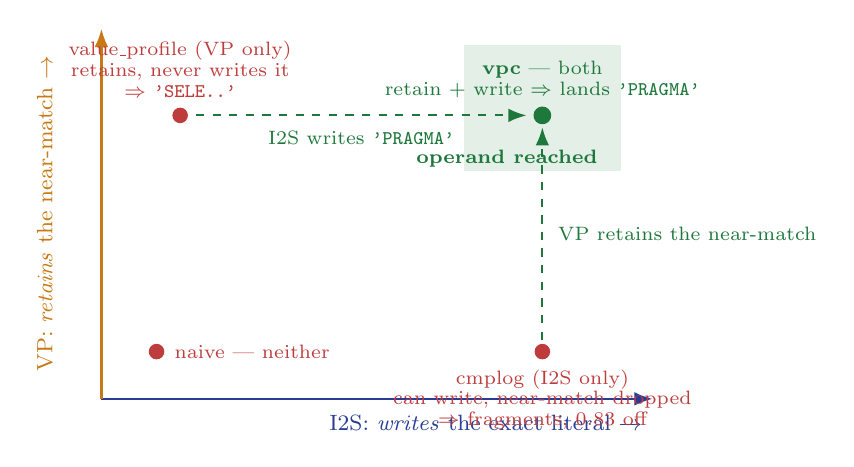
\begin{tikzpicture}[font=\footnotesize,>=Latex]
% two-axis joint-necessity plot: x = I2S capability (writes the exact literal),
%                                y = VP capability  (retains the near-match)
\draw[->,i2sc,thick] (0,0) -- (7.0,0) node[below=2pt,i2sc,anchor=north east]{I2S: \emph{writes} the exact literal $\rightarrow$};
\draw[->,vpcol,thick] (0,0) -- (0,4.7);
\node[vpcol,rotate=90,anchor=south] at (-0.5,2.35) {VP: \emph{retains} the near-match $\rightarrow$};
% pass region (top-right corner)
\fill[winc!12] (4.6,2.9) rectangle (6.6,4.5);
\node[winc] at (5.15,3.05) {\scriptsize\textbf{operand reached}};
% the four arms
\filldraw[losc] (0.7,0.6) circle (2.6pt) node[right=3pt,losc,align=left]{\scriptsize naive --- neither};
\filldraw[losc] (5.6,0.6) circle (2.6pt) node[below=3pt,losc,align=center]{\scriptsize cmplog (I2S only)\\[-2pt]\scriptsize can write, near-match dropped\\[-2pt]\scriptsize $\Rightarrow$ fragments, $0.83$ off};
\filldraw[losc] (1.0,3.6) circle (2.6pt) node[above=3pt,losc,align=center]{\scriptsize value\_profile (VP only)\\[-2pt]\scriptsize retains, never writes it\\[-2pt]\scriptsize $\Rightarrow$ \texttt{'SELE..'}};
\filldraw[winc] (5.6,3.6) circle (3pt) node[above=3pt,winc,align=center]{\scriptsize\textbf{vpc} --- both\\[-2pt]\scriptsize retain $+$ write $\Rightarrow$ lands \texttt{'PRAGMA'}};
\draw[->,winc,thick,dashed] (5.6,0.75) -- (5.6,3.45) node[midway,right=2pt]{\scriptsize VP retains the near-match};
\draw[->,winc,thick,dashed] (1.2,3.6) -- (5.4,3.6) node[midway,below=2pt]{\scriptsize I2S writes \texttt{'PRAGMA'}};
\end{tikzpicture}\\[2pt]
{\footnotesize Each single technique supplies one capability and stays outside the
\textcolor{winc}{operand-reached} corner: \texttt{cmplog} can write the literal but
without the gradient its half-right seed is dropped, so the keyword never lands
($0.83$ residual); \texttt{value\_profile} retains near-misses but can't write the
exact bytes. Only \texttt{vpc} both retains the partial match \emph{and} writes it,
so \texttt{'PRAGMA'} is reached (residual $0.83\!\to\!0$). (sqlite3/16001, real metrics.)}
\end{center}

\paragraph{Sub-cases.} Of the 18 branches, 15 are the plain operand-reach form
above; 2 (\texttt{joint\_fixed\_offset\_literal\_presence}, harfbuzz/6858,7245)
gate on a fixed-offset FOURCC where the blocking arm carries junk at the offset
(confirmed by \texttt{signed\_target\_enrich}$\ge 1.0$ instead, the
operand-enrichment route); 1 (\texttt{joint\_value\_gradient\_closure},
libxml2/7326, operand \texttt{'<![CDATA['}) is the same operand-reach on a longer
string token scored purely on \texttt{value\_distance\_reached}. The mechanism ---
I2S writes the literal, the gradient retains the near-match --- is identical; only
the measurable proxy differs.

\paragraph{Caveat on the proxy.} \emph{Every} category-1 operand is itself a
literal the I2S stage could in principle substitute (keywords / table tags:
\texttt{PRAGMA}, \texttt{OS/2}, \texttt{loca}, \texttt{CPAL}, \texttt{CFF},
\texttt{<![CDATA[}). So the discriminating fact is never ``cmplog can't write
it'' but ``cmplog's corpus doesn't \emph{retain} a seed that lands it'' --- which
is exactly the retention the gradient adds. The reading is clearest where the
evidence says so outright (sqlite3/16001: cmplog ``cannot retain and refine''
near-keywords). It is least intuitive when the operand is a bare 4-byte tag the
parser checks early, e.g.\ \mbox{harfbuzz/5602} (operand \texttt{'OS/2'},
\texttt{cmp\_min\_distance}$=0.5$): there a \texttt{vpc}-vs-\texttt{cmplog}
distance gap is surprising precisely because \texttt{cmplog} has I2S, so that
branch rests entirely on the retention reading rather than on any field-level
distance. The \texttt{value\_distance} number measures operand presence, not the
downstream-field tuning an earlier draft implied.

% =====================================================================
\section*{2.\ \ Structural assembly depth under joint necessity \hfill {\normalsize\texttt{joint\_assembly\_depth} ($n=9$)}}
Here the second key is not a precise value but \emph{more structure / depth}. The
gate sits behind interlocking fields. I2S places the exact tags/literals that keep
the parser on a valid path --- the gradient-only arm (\texttt{value\_profile})
places \emph{zero} of them and dies early --- but a single I2S pass does not
\emph{grow} the input far enough, so \texttt{cmplog} assembles a partial structure
and stalls. Only \texttt{vpc} climbs the gradient to build deeper. This shows up two
ways: more loop \emph{iterations} (\texttt{depth\_reach}, 2 branches) or more bytes
\emph{assembled} (\texttt{seed\_size\_and\_tags}, 7 branches). The clearest gate is an
iteration one:

\begin{lstlisting}[style=c]
// harfbuzz  src/hb-ot-post-table.hh : line 255   (verbatim source line)
//   the resolving (false) side needs BOTH keys on one line: the exact version
//   magic (I2S plants 0x00020000) AND glyph in bounds (glyph < glyphNameIndex->len),
//   which the gradient reaches by driving the post-table glyph loop deeper per seed
if (version != 0x00020000 || glyph >= glyphNameIndex->len)  // <-- blocker (harfbuzz/5616)
    return false;
\end{lstlisting}
\noindent{\footnotesize Verbatim source line at \texttt{post-table.hh:255}: one line
carries \emph{both} techniques --- \texttt{0x00020000} is the I2S literal, and
\texttt{glyph < glyphNameIndex->len} is the bound the gradient closes by iterating.}

\noindent\textit{Stripped to its two keys} (simplified for clarity --- same gate,
the loop the real one-liner hides made explicit):
\begin{lstlisting}[style=c]
// Category 2A -- iteration DEPTH (simplified from harfbuzz/5616, post-table.hh:255)
if (version != 0x00020000)         // KEY 1 (I2S): exact 4-byte version magic
    return BLOCKED;                //   value_profile never plants it -> blocks here
while (i < glyph) walk(i++);       // KEY 2 (gradient): the index only comes in-bounds
                                   //   after the parser iterates this loop deep enough
if (glyph < glyphNameIndex->len)   // cmplog enters the loop ONCE (depth ~1) and stalls;
    return RESOLVED;               //   only vpc re-enters + iterates deep (depth ~157x)
return BLOCKED;
\end{lstlisting}

\noindent\textbf{How we know it is really joint.} For an iteration gate we run each
arm's corpus through the instrumented coverage binary and count, per seed, how many
times the blocker line executes (\texttt{depth\_reach}). \texttt{value\_profile}
(gradient, no I2S) never places the version magic and never reaches the line; the
discriminating signal is that \texttt{vpc} drives the line far deeper than the
I2S-only \texttt{cmplog}.

\metricbox{depth\_reach}
{\texttt{depth\_lift} = vpc / cmplog per-seed executions of the blocker line; \texttt{winner\_depth}, \texttt{loser\_depth}; \texttt{winner\_deeper} (bool)}
{depth\_lift >= 1.5 AND winner\_deeper == true}
{harfbuzz/5616 (\texttt{post-table.hh:255}) --- \texttt{vpc} executes the gate line \texttt{winner\_depth}$=157.2$ times per seed against the \texttt{cmplog} arm's \texttt{loser\_depth}$=1.0$ (\texttt{depth\_lift}$=157.2$): the gradient retains the near-miss inputs that let the corpus re-enter and iterate the gated loop, while I2S alone touches it once and stalls.}

\paragraph{The other (and more common) form: byte growth.} For 7 of the 9 branches
the depth is raw size, scored by \texttt{seed\_size\_and\_tags} (rule \texttt{vp\_tags <
0.3 AND size\_lift >= 1.3}). Real example harfbuzz/6814: the gradient-only arm
assembles \emph{no} table tags (\texttt{vp\_tags}$=0$, so I2S is necessary), while
\texttt{vpc} grows the input $2.4\times$ past the I2S-only arm
(\texttt{size\_lift}$=2.44$):

\begin{lstlisting}[style=c]
// Category 2B -- assembly SIZE (simplified from harfbuzz/6814; cf. shape-normalize.cc:196)
if (!has_tag(font,"cmap") || !has_tag(font,"GSUB"))  // KEY 1 (I2S): exact table tags
    return BLOCKED;                 //   value_profile assembles 0 tags -> blocks (vp_tags=0)
record = build_full_table(font);    // KEY 2 (gradient): the WHOLE record must be grown
if (record_complete(record))        //   cmplog grows ~248 B (partial) and stalls;
    return RESOLVED;                //   only vpc grows it ~604 B (2.4x) -> resolves
return BLOCKED;
\end{lstlisting}

\begin{center}
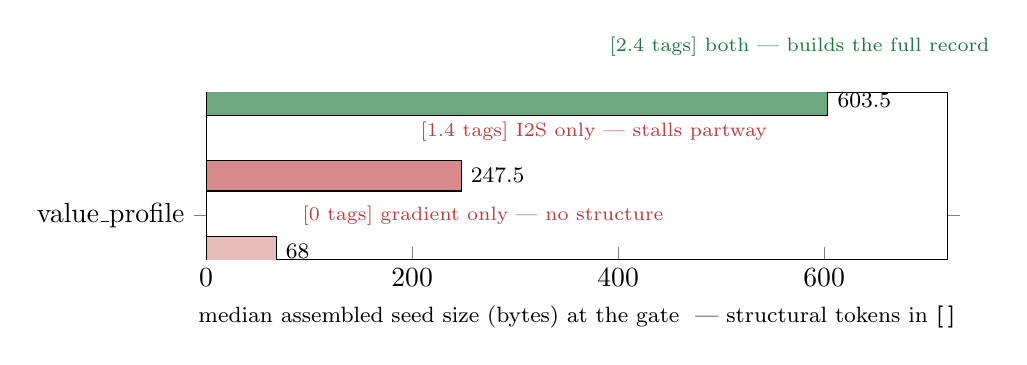
\begin{tikzpicture}
\begin{axis}[
  width=11cm, height=3.7cm, xbar, xmin=0, xmax=720,
  bar width=11pt, enlarge y limits=0.55,
  symbolic y coords={value\_profile, cmplog, vpc},
  ytick=data, xtick={0,200,400,600},
  nodes near coords, every node near coord/.append style={font=\footnotesize},
  xlabel={\footnotesize median assembled seed size (bytes) at the gate \ ---\ structural tokens in \textbf{[\,]}},
]
\addplot[fill=losc!35] coordinates {(68,value\_profile)};
\addplot[fill=losc!60] coordinates {(247.5,cmplog)};
\addplot[fill=winc!65] coordinates {(603.5,vpc)};
\end{axis}
\node[font=\scriptsize,anchor=west] at (1.1,0.55) {\textcolor{losc}{[0 tags] gradient only --- no structure}};
\node[font=\scriptsize,anchor=west] at (2.6,1.62) {\textcolor{losc}{[1.4 tags] I2S only --- stalls partway}};
\node[font=\scriptsize,anchor=west] at (5.0,2.7) {\textcolor{winc}{[2.4 tags] both --- builds the full record}};
\end{tikzpicture}\\[-1pt]
{\footnotesize The gradient-only arm (\texttt{value\_profile}) places no tags and
stays tiny; I2S-only (\texttt{cmplog}) gets the tags but only a partial
structure; \texttt{vpc} grows it $2.4\times$ larger to reach the deep gate.
(harfbuzz/6814, real metrics.)}
\end{center}

% =====================================================================
\section*{At a glance}
\begin{center}\small
\begin{tabular}{@{}p{3.25cm}c>{\raggedright\arraybackslash}p{4.35cm}>{\raggedright\arraybackslash}p{4.45cm}@{}}
\toprule
\textbf{Category} & \textbf{$n$} & \textbf{Tool / metric} & \textbf{What the gradient adds} \\
\midrule
value\_distance\_closure & 18 & seed\_size\_and\_tags $+$ value\_distance\_reached / \texttt{size\_lift}, \texttt{distance\_closure\_ratio} & \emph{retain} the near-match so I2S lands the exact operand --- reached in the joint corpus, absent from the I2S-only one (incl.\ 2 fixed-offset-presence, 1 string-token sub-cases) \\[2pt]
assembly\_depth & 9 & seed\_size\_and\_tags / \texttt{vp\_tags}, \texttt{size\_lift} & grow a larger \emph{structure} I2S alone never assembles (incl.\ 2 iteration-depth via \texttt{depth\_reach}) \\
\midrule
\textbf{VPC-pro total} & \textbf{27} & \multicolumn{2}{>{\raggedright\arraybackslash}p{9.5cm}@{}}{all share joint necessity: \texttt{cmplog} \emph{and} \texttt{value\_profile} each block alone; only \texttt{vpc} resolves} \\
\bottomrule
\end{tabular}
\end{center}

\noindent\footnotesize Counts and example metrics are from
\texttt{bench/dataset.jsonl}; verify rules are the deterministic arbiter rules
(no LLM in the decision). The joint family is exclusive by its deciding pair
\mbox{$p\succ c \,\wedge\, p\succ v$} (\texttt{value\_profile\_cmplog} beats both
single arms), so a branch resolvable by either technique alone never lands here.
harfbuzz corpora live on the other server; the cited metrics were scored there
and merged into the dataset.
\end{document}
